% Todo Betere titel vinden
\chapter{Onderzoek: Externe bibliotheken gebruiken en het gevaar hiervan}\label{ch:externeGevaren}
Om een houvast te hebben in het ontwikkelen van een methode voor het analyseren van externe bibliotheken op kwetsbaarheden moet er een onderzoek gedaan worden over de theorie over het gebruik van externe bibliotheken, het gevaar en op welke manier er veilig mee gewerkt kan worden. De onderzoeksvraag voor dit onderzoek luidt dan ook: Wat is het effect van het gebruik van externe bibliotheken bij het ontwikkelen van software, welke gevaren brengt dit met zich mee en wat kan er gedaan worden om deze gevaren te minimaliseren?". Deze onderzoeksvraag is op te delen in de volgende deelvragen die ieders in een sectie worden beantwoord met als doel een conclussie te kunnen geven die als input te gebruiken is voor het onderzoek naar een methode voor SOUP analyses binnen EagleScience.

\begin{itemize}
    \item Hoeveel gebruik wordt er gemaakt van externe bibliotheken bij de ontwikkeling van applicaties?
    \item Waarom worden externe bibliotheken gebruikt in het ontwikkelen van software?
    \item Wat zijn potienteel gevaren die het gebruik van externe bibliotheken kunnen introduceren?
    \item Hoe kan er voorkomen worden dat er kkwetsbaarheden onstaan in een applicatie die gebruik maakt van externe bibliotheken?
    \item
\end{itemize}

\section{Hoeveel gebruik wordt er gemaakt van externe bibliotheken bij de ontwikkeling van applicaties?}
Software wordt tegenwoording voor een groot deel vervaardigd door gebruik te maken van open source-code. Volgens een onderzoek gedaan door Synopsys\footnote{Synopsys is een bedrijf dat zich bezig houd met de ontwikkeling en verification van semiconductoren. Daarnaast ontwikkeld het tools voor verschillende taken in het domein software veiligheid. } (https://www.synopsys.com/software-integrity/resources/analyst-reports/open-source-security-risk-analysis.html?intcmp=sig-blog-ossra1) bestond in 2020 98\% van de 1546 geanalyseerde codebases uit opensource componenten. Daarnaast hadden ze gevonden dat 84\% van deze codebases minimaal één kwetsbaarheid bevat met een gemiddelde van 158 kwetsbaarheden. De gemiddelde kwetsbaarheid was 2.2 jaar oud.

Ook al is dit onderzoek gedaan door een bedrijf wat zelf tools verkoopt om kwetsbaarheden op te sporen en dus de cijfers in hun voordeel zijn afgerond. Is het probleem van kwetsbaarheden in bibliotheken van derden zeer groot. Als we onderzoeken van andere bedrijven bekijken komen die op een ongeveer dezelfde getallen. TideLift, een bedrijf dat zich inzet voor verbeteren van het gebruik en veilig gebuik van OpenSource software,  claimde in 2019 al dat 92\% van de ontwikkelde applicaties Open Source componenten bevat.

https://www.zdnet.com/article/its-an-open-source-world-78-percent-of-companies-run-open-source-software/



\section{Waarom worden externe bibliotheken gebruikt in het ontwikkelen van software?}
Bibliotheken zorgen over het algemeen ervoor dat herhalende taken die applicaties uit moeten voeren éénmalig wordt ontwikkeld en vervolgens voor meerdere projecten/applicaties in te zetten is. Op deze manier wordt ontwikkeltijd gewonnen omdat herhalende source-code geimporteerd kan worden en niet opnieuw geschreven hoeft te worden. Doordat het op een enkele plaats gedefineerd staat hoeft dit ook in het geval van een aanpassing maar op een enkele plek aangepast te worden Dit scheeld wederom tijd, maar ook potentieel fouten omdat de aanpassing niet overal hoeft te worden doorgevoerd. Het gebruik van bibliotheken is dus bijna niet weg te denken gezien de druk die op het ontwikkelen van software staat. Een stap verder is het gebruik van externe bibliotheken welke ervoor zorgen dat er om dezelfde redenen als hierboven nog minder ontwikkeltijd nodig is omdiezelfde taken te kunnen gebruiken echter wordt de bibliotheek niet door ontwikkelaars zelf ontwikkeld maar door een externe partij. Naast dat het gebruik van externe bibliotheken tijdswinst en dus de kosten voor het ontwikkelen van een applicatie kan verminderen zijn er nog een aantal voordelen die het benoemen waard zijn op het moment dat er veel gebruikte externe bibliotheken gebruikt worden in het ontwikkelproces: Als een bibliotheek gebruikt wordt door een groot aantal andere bedrijven ontstaat hier veel kennis over, wat resulteert in veel documentatie en support en een door de comunity ondersteunde standaard wat op zijn beurt weer helpt in het makkelijker op kunnen leiden van nieuw personeel. Daarnaast is er het feit dat als er door een 'grotere' community een biobluitheek gebruikt wordt deze ook vaker getest zal zijn. waarmee de functionele betrouwbaarheid verhoogd wordt.




\section{Wat zijn potienteel gevaren die het gebruik van externe bibliotheken kunnen introduceren?}
Hoewel de voordelen die hierboven beschreven zijn enorm kunnen zijn voor bedrijven die software ontwikkelen. Zijn er ook een aantal nadelen te benoemen waarvan de grootste wel is dat er potentieel kwetsbaarheden kunnen worden geintroduceert in de applicatie die niet direct kunnen worden gezien door ontwikkelaars die de bibliotheken gebruiken. Deze kwetsbaarheden kunnen zich op meerdere manieren manifesteren in de vorm van een "Supply Chain Attack". Waarbij zoals de naam al doet vermoeden er een aanval plaats vindt middels software die zich in de dependencies bevindt deze aanval kan op verschillende manieren plaatsvinden maar hebben meestal als doel dat er op een één of andere manier data bemachtigd wordt of anders de functionaliteit van de doel applicatie op een dusdanige manier wordt aangetast dat deze in het voordeel is van de aanvallers. Een probleem met dit soort aanvallen is veelal dat deze lange tijd onopgemerkt kunnen blijven (SolarWinds attack) omdat externe bibliotheken niet vaak worden gecheckt op juistheid. En op het moment dat ze al opgemerkt worden en er een verslag is gemaakt in een Vulnerablitiy database (NIST, NVD, Mitre) Deze ook nog door andere bedrijven die dezelfde bibliotheek met de zelfde versie wordt gebruikt waarbij deze bedrijven ook kwetsbaar zijn. Uit onderzoek van Sonartype blijkt dat een groot deel van de applicaties niet worden bijgewerkt of veelal niet op de juiste manier zodat er altijd een kwetsbaarheid zal blijven bestaan.





\section{Hoe kan er voorkomen worden dat er kkwetsbaarheden onstaan in een applicatie die gebruik maakt van externe bibliotheken?}
Hoewel er veel bedrijven en instanties zich verantwoordelijk voelen, dan al niet voor winst, om het mogelijk te maken om vilige software te ontwikkelen. Bestaat de OWASP puur en alleen om dit te doen op een vrijwillige basis. Zei doen dit door awareness te kweken over het veilig ontwikkelen van software. Eén van de belangrijkste methoden die zij hebben is de OWASP top 10 waarin iedere 5 jaar een lijst wordt gepresenteerd met de meest ktitsiche aspecten voor het ontwikkelen van veilige software. In 2021 stond op plaats A06:2021 een item over het


\section{Hoeveel gebruik wordt er gemaakt van externe bibliotheken?}

\section{OWASP}

\section{Waarom potentieel gevaarlijk}

\section{Hoe moet het opgelost worden}


zijn de resultaten toch wel beangstigend.



[NOTE:] Is dit hoofdstuk nog wel relevant?????
Dit hoofdstuk beschrijft het onderzoek wat gedaan is om meer inzicht te krijgen in het doen van een SOUP-analyse. Als eerst wordt de onderzoeksvraag ontleed in te beantwoorden deelvragen. Daarna zal er wordt iedere deelvraag beantwoord om vervolgens tot een conclusie te komen welke de onderzoeksvraag beantwoord.


\section{Onderzoeksvragen} \label{sec:SOUPOnderzoeksvragen}
De onderzoeksvraag die als startpunt van dit onderzoek geld is:"Hoe kunnen we externe bibliotheken op een veilige manier gebruiken?" of "Hoe kan SOUP op een effectieve manier worden geanalyseerd en hoe maakt dit software veiliger?". Uit deze hoofdvraag kunnen de volgende deelvragen worden ontleed:
\begin{itemize}
    \item Wat is veilige software?
    \item Wat is SOUP?
    \item Wat dragen externe bibliotheken en dus ook potentieel SOUP bij aan de ontwikkeling van software?
    \item Wat zijn de gevaren van het gebruik van SOUP?
    \item Wordt er ergens bijgehouden of een dependency/component) een kwetsbaaheid bevat?
\end{itemize}

%Goed verhaal over supplychain Attacks : https://learning.oreilly.com/library/view/alice-and-bob/9781119687351/c01.xhtml#head-2-27


\section{Wat is veilige software?}
Veilige software is software dat ontworpen is met onder andere de CIA Triad(confidentiality(vertrouwelijkheid), integrity(integriteit), and availability(beschikbaarheid)) figuure:~\ref{fig:CIA}) in het oog. Dit wil zeggen dat de informatie binnen een applicatie aan de volgende zaken moet voldoen.
\begin{figure}[H]
    \centering
    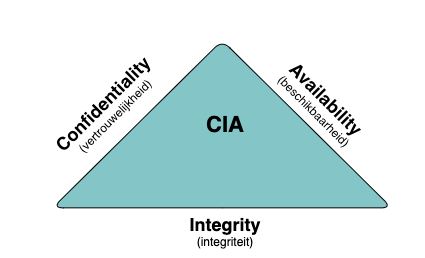
\includegraphics[width=6cm]{gfx/CIA}
    \caption{C.I.A Triad}
    \label{fig:CIA}
\end{figure}

\begin{itemize}
    \item \textbf{vertrouwelijk}: Alleen degene die het recht hebben om de informatie in te zien kunnen deze informatie inzien.
    \item \textbf{integer}: De informatie welke opgeslagen en gebruikt wordt is daadwerkelijk de juiste informatie
    \item \textbf{beschikbaar}: De informatie is beschikbaar op het moment dat het nodig is.
\end{itemize}
Deze drie kernwoorden zorgen ervoor dat als er goed over nagedacht is tijdens de ontwerpfase een goed beeld kan ontstaan hoe een goede applicatie ontwikkeld dient te worden.

Daarnaast zijn er nog een aantal lagen van veiligheid die in een applicatie gebouwd kunnen worden.
Een binnen EagleScience toegepast voorbeeld zou zijn(zie figuur~\ref{fig:veiligheidslagen}):

\begin{figure}[H]
    \centering
    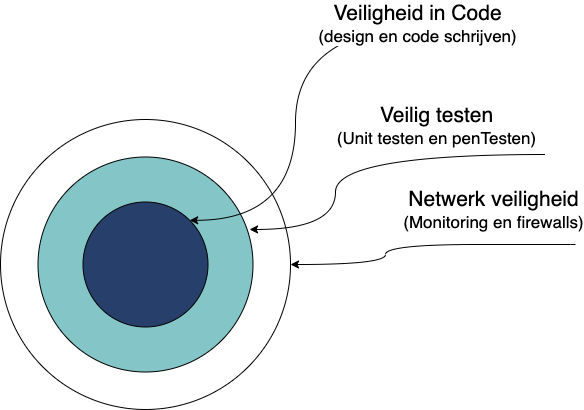
\includegraphics[width=6cm]{gfx/veiligheids lagen}
    \caption{Veiligheids lagen}
    \label{fig:veiligheidslagen}
\end{figure}

\begin{itemize}
    \item \textbf{Tijdens de ontwikkeling van software} is het van belang om de juiste security requirements op te nemen in de requirements documentatie, En dat deze middels, veilige ontwerp concepten worden toegepast,'secure coding tactics', (penetration)testing door verschillende personen en tools worden nageleefd.
    \item \textbf{Tijdens de levensduur van de applicatie} dient de monitoring, op netwerkverkeer en events goed in de gaten gehouden worden dan al niet middels tools en triggers.
    \item \textbf{fysieke beveiliging} De laatste vorm van beveiging zijn daadwerkelijk sleutels op fysieke sloten van de server ruimte en de beslissingen wie deze sleutels heeft.
\end{itemize}
Door deze drie lagen te hanteren heeft EagleScience het ontwikkelen van veilige software in de hand. Daarnaast wordt de OWASP TOP-10 als guideline gebruikt om te zien op welke zaken er gelet dient te worden. De OWASP Top-10 wordt iedere 5 jaar uitgegeven en geeft een beeld van de meest vookomende veiligheidslekken. in 2021 staat op plaats 6 een item over kwetsbare en oude componenten. \cite{Kohnfelder2021}


\section{Externe Componenten}\label{sec:software-of-unkown-provenance}
Binnen EagleScience bestaat er geen applicatie dit op enig manier gebruik maakt van extern ontwikkelde componenten. Componenten in deze zin zijn ook de runtime\-omgevingen zoals Operatingsystems dan al niet middels een docker container en programeertalen. Echter de componenten waar het in dit onderzoek over gaat zijn de packeges en dependencies die gebruikt worden voor de door EagleScience ontwikkelde applicaties. Met name bibliotheken die veel gebruikte taken vergemakkelijken worden veel ingezet. Hierbij kan gedacht worden aan frameworks voor de frontend als Angular of een framework als Play welke gebruikt wordt als basis voor onze backend applicaties. Vaak bestaan dependencies uit meerdere lagen dus een dependency die direct gebruikt wordt door een applicatie kan zelf ook weer dependencies hebben Wat het doorzoeken van kwetsbaarheden lastiger maakt. Gebruikte dependencies wordt in sommige velden ook SOUP genoemd.

\subsection{Wat is Software of Unkown Provenance(SOUP)?}\label{subsec:wat-is-soup?2}
De term SOUP komt oorspronkelijk de wereld van de ontwikkeling van medische software en staat voor "Software Of Unkown Provenance".
SOUP wordt gezien als een software component dat al ontwikkeld is en beschikbaar is gesteld voor gebruik door een instantie anders dan de gebruiker zonder dat de bewijzen zijn over de manier van ontwikkeling als de kwaliteit van de software.
Hierdoor is het dus niet duidelijk welk process er is gevolgt tijdens het ontwikkelen en daarmee dus ook de (medische)veiligheid niet is aan te tonen.
De term wordt nu steeds vaker gebruikt in de algemene software ontwikkel kringen om aan te geven dat er van een betreffent software component(framework, bibliotheek, etc.) niet bekend is hoe het ontwikkeld, getest is.
Hierdoor is er dus geen zekerheid dat het component kwetsbaarheden kan bevatten.
Kwetsbaarheden in deze zin zijn dan voornamelijk lekken of veranderingen van functionaliteiten binnen een software.

\sebsection{Wat dragen externe bibliotheken bij aan de ontwikkeling van software??}
Zoals hierboven beschreven zorgen externe bibliotheken ervoor dat veel gebruikte functies niet opnieuw geschreven hoeven te worden. Wat mits er een goede documentatie voor bestaat veel tijd en dus geld kan besparen. Een ander voordeel kan zijn dat als een veelgebruikte framework wordt gebruikt nieuwe collega's makkelijker aan een project kan werken zonder een lang inwerk traject.
De voornaamste redenen om bibliotheken te gebruiken is het verminderen van het herhaaldelijk schrijven van code om basis functionaliteiten in een applicatie te krijgen. En Daarmee wordt de ontwikkeltijd verminderd. Het gebruik van bibliotheken is tegenwoordig niet meer weg te denken uit de ontwikkelstrategie van een bedrijf. Deels omdat er een standaard is waarmee gewerkt wordt, wat op zijn beurt het aannemen en opleiden van personeel vergemakkelijkt. Daarnaast hebben veel gebruikte bibliotheken een 'community' waar vragen gesteld kunnen worden om zo moeilijkheden te verminderen. Een nadeel zoals hierboven is beschreven is dat het niet altijd duidelijk is hoe veilig een bibliotheek is.


\subsection{Hoe relateert SOUP zich met het ontwikkelen van veilige software?}\label{subsec:hoe-relateert-soup-zich-met-het-ontwikkelen-van-veilige-software?}
%Bron: Contrast Security >> https://cdn2.hubspot.net/hub/203759/file-1100864196-pdf/docs/Contrast_-_Insecure_Libraries_2014.pdf
%Bron: https://www.veracode.com/sites/default/files/pdf/resources/reports/state-of-software-security-open-source-edition-veracode-report.pdf
externe bibliotheken worden veelvuldig gebruikt. Uit een onderzoek van VeraCode, een bedrijf dat een platform aanbied om software te ontwikkelen, kan opgemaakt worden dat 96\% van alle ontwikkelende bedrijven gebruik maakt van opensource componenten. Uit hetzelfde onderzoek komt naar boven dat het probleem van kwetsbaarhden niet zozeer in de direct gebruikte frameworks zitten maar eerder in de dependencies van deze frameworks de zogenaamde translative bibliotheken.


\section{Hoe kan het gebruik van SOUP gevaarlijk zijn?}\label{sec:hoe-kan-het-gebruik-van-soup-gevaarlijk-zijn?}
Zoals inmiddels duidelijk bestaat een software component uit een mix van eigen geschreven source code en source code die geschreven staat in bibliotheken dan al niet van derden, zogenoemde depenencies. Deze regel geldt dus niet alleen voor de applicaties die door EagleScience is geschreven, maar dan ook voor de dependencies die gebruikt worden voor de geimporteerde dependency. Dit gaat resursief door totdat we bij dependencies aankomen die zelf geen dependencies gebruiken om hun taak te voltooien. Dit wordt ook wel een dependency tree genoemd. figuur ~\ref{fig:dependency-tree} geeft een verkapte versie weer waarin geillusteerd wordt hoe snel het aantal dependencies optelt.
\begin{figure}[H]
    \myfloatalign
    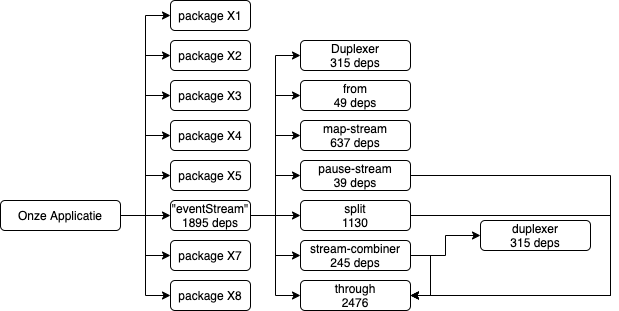
\includegraphics[width=12cm]{gfx/dependencyTree}
    \caption{Dependency tree}\label{fig:dependency-tree}
\end{figure}

\section{Wordt er ergens bijgehouden of een (dependency/component) een kwetsbaaheid bevat?}\label{sec:item-wordt-er-ergens-bijgehouden-of-een-dependency/component)-een-kwetsbaaheid-bevat?}
Naast de OWASP zijn er nog een aantal instanties die zich bezighouden met het veilighouden van software. Vaak is dit het verzamelen van kwetsbaarheden en deze vind en kenbaar maken aan het publiek. Twee instituten die samenwerken zijn MITRE en Information TechnologyLab van het NIST\footnote{National Institute of Standards and Technology: Instituur onder amerikaanse regering die verschillende onderzoeken doen op het het gebied van technologie}TL van

\subsection{CVE Databases, MITRE, NIST, NVD}\label{subsec:mitre-nist-nvd}
CVE staat voor Common Vulenerabilities en Exposures wat een database waarin kwetsbaarheden staan die gevonden zijn in de verschillende systemen.
Deze Database wordt voornamelijk bijgehouden door het bedrijf MITRE dat met subsidie van de US Division of Homeland Security werkt aan het kenbaar maken van lekken in software\footnote{Software wordt hier gezien in de ruimste zin van het woord hierbij hoort: Operating systems, open en closed source software. maar ook frameworks en bibliotheken.}.
De CVE's die in deze database staan worden vervolgens geannalyseerd door het NIST(National Institute os Standards and Technology) en voorzien van een CVSS\footnote{Common Vulnerability Score System is een gestandardiseerde manier om een score aan een kwetsbaarheid toe te kennen waarop in een enkel oog opslag te zien is hoe rieel een risico is.} score en geplaats in de NVD-database.
Zowel de database van MITRE (https://cve.mitre.org) als NIST (https://nvd.nist.gov) zijn publiekelijk toegankelijk.

\subsection{OWASP}\label{subsec:owasp}
Naast het bijhouden van CVE's in database is het creëren van awareness net zo belangrijk.
Een instantie die zich bezig houd hier mee is OWASP(Open Web Application Security Project) die awareness creëert door ideree 5 jaar een Top-10 uit te brengen met daarin de meest voorkomende en dreigende kwetsbaarheden die ze gevonden hebben in een dataset wat opgebouwd is uit inzendingen van 500+ onderzoekers van 40+ bedrijven die samen meer dan 100.000 API's en web applicaties hebben onderzocht.
In de top 10 die hieronder samengevat weer wordt gegeven wordt er een score meegegeven over hoe makkelijk een lek is te ontdekken en welk mate van risico de kwetsbaarheid heeft.
%Bronnen:
%https://www.imperva.com/learn/application-security/cve-cvss-vulnerability/
%http://owasp.org

